\documentclass[../main.tex]{subfiles}

\begin{document}

In general we study the HeNe laser using the following experimental setup (figure \ref{fig:general_setup}).
\begin{figure}[H]
    \centering
    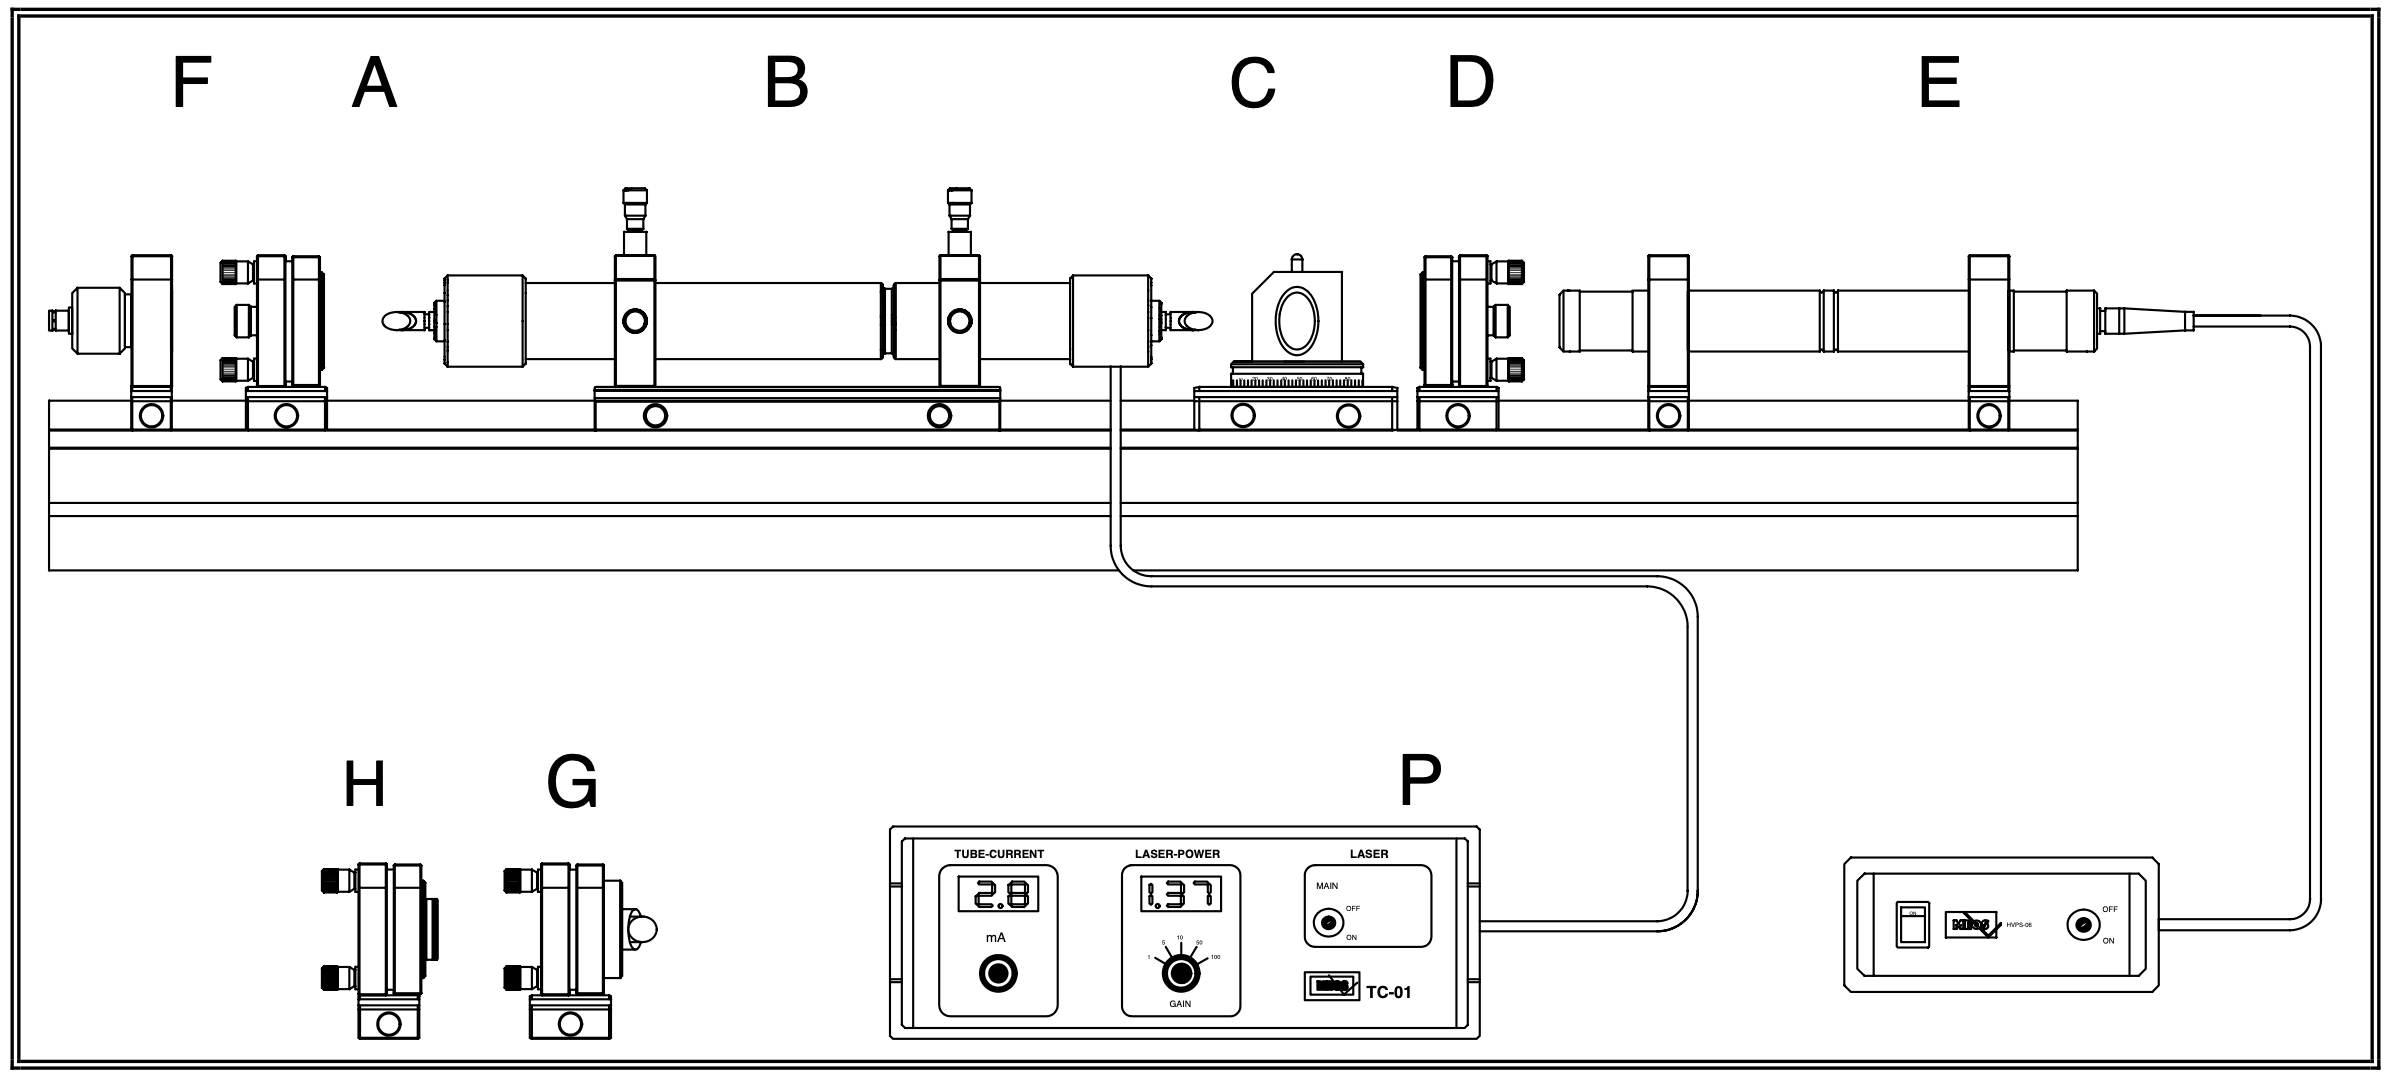
\includegraphics[width=0.8\linewidth]{Bilddateien/Versuchsaufbau/general_setup.png}
    \caption{General experimental setup with components (A) to (H) and (P).}
    \label{fig:general_setup}
\end{figure}
Module (A) contains the left cavity mirror, which can be screwed into the module. Module (B) contains the main laser module a.i. the active medium, which will be moved in displacements $\delta L$ later on. Module (D) closes the main laser setup and contains the right cavity mirror. Module (A), (B) to (D) are the most important changeable parameters in our experiment, with the power module (P) in addition. 

The prisms are given by (C) (Birefringent tuner), (G) (Littrow prism tuner) and (H) (Fabry Perot etalon), the laser adjustment is achieved with the help of module (E) (Pilot laser). For power detection we use the photomodule (F). 


\subsection{Dependance of output power from laser discharge current}
    \subfile{4-Auswertungsteile/4-2-Auswertungsteil.tex}

\subsection{Dependance of ouput power from position of main laser tube}
    \subfile{4-Auswertungsteile/4-3-Auswertungsteil.tex}

\subsection{Optical stability}
    \subfile{4-Auswertungsteile/4-4-Auswertungsteil.tex}

\subsection{Wavelength selection}
    \subfile{4-Auswertungsteile/4-5-Auswertungsteil.tex}

\subsection{Mode selection}
\subfile{4-Auswertungsteile/4-6-Auswertungsteil.tex}

\end{document}